
\subsection{Ecualizador de Fase}


\begin{figure}[H]
	\centering
	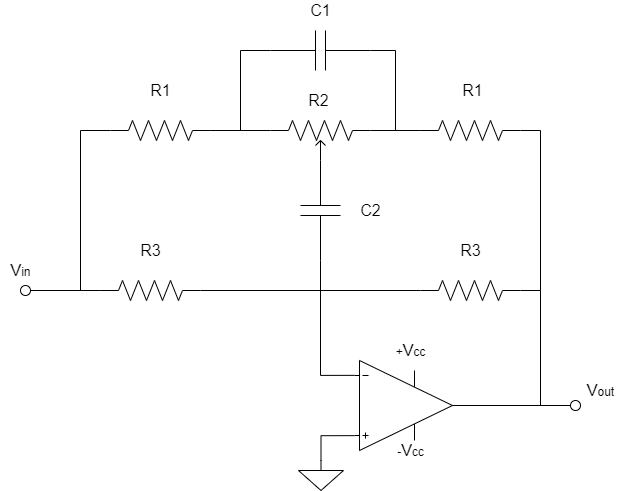
\includegraphics[width=0.6\textwidth]{../Ejercicio4-EcualizadorDeFase/Informe/Ecualizador de Fase.png}
	\caption{Circuito Ecualizador de Fase}
\end{figure}


\subsection{Análisis matemático}

Para analizar el circuito propuesto, se opto por reemplazar la resistencia variable $R_2$ por dos resistencias las cuales llamaremos 
$R_{21}$ y $R_{22}$, relacionadas por un coeficiente $\delta$. 
De esta forma será más fácil poder resolver el circuito propuesto, entonces definimos:

\begin{align}
		R_{21} &= R_2  \delta \\
		R_{22} &= R_2  (1 - \delta)
\end{align}


\begin{figure}[H]
	\centering
	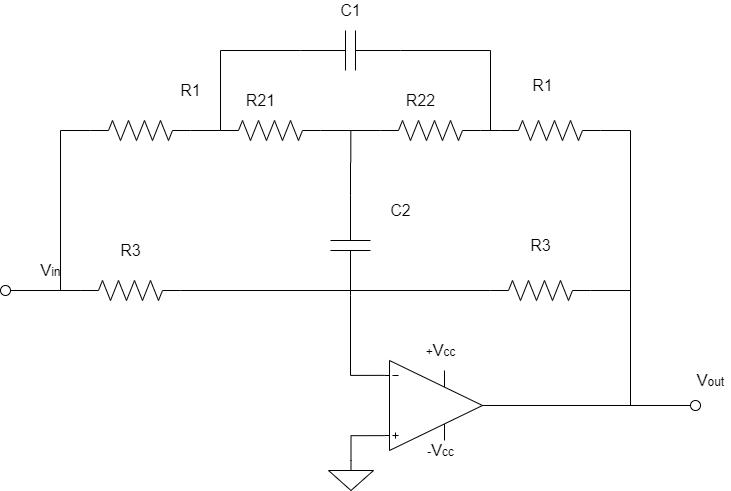
\includegraphics[width=0.6\textwidth]{../Ejercicio4-EcualizadorDeFase/Informe/EcSinPot.png}
	\caption{Modelo matemático}
\end{figure}

Se utilizo el reemplazo de impedancia de configuración 
triangulo a estrella y luego una transformación de configuración
 estrella a triangulo como se muestra en las imágenes [\ref{1reemplazo}]
  y [\ref{2reemplazo}]  para poder simplificar el circuito lo más posible.
Para el primer reemplazo se usaron las siguientes ecuaciones:

\begin{align*}
		Z_{AB} &= \frac{1}{sC_1} \\
		Z_{BC} &= R_{22} \\
		Z_{CA} &= R_{21}
\end{align*}
A partir de la misma, se realiza una transformación de parámetros triángulo
a estrella, de tal manera de simplificar nuestro circuito.
 Se hacen las 
siguientes consideraciones:

\begin{align*}
	Z_{eq} &= Z_{AB} + Z_{BC} + Z_{CA}
\end{align*}

El desarrollo matemático realizado fue el siguiente: \par 

\begin{align}
	Z_{A} &= \frac{Z_{AB}+Z_{CA}}{Z_{eq}} \\
	Z_{B} &= \frac{Z_{AB}+Z_{BC}}{Z_{eq}}  \\
	Z_{C} &= \frac{Z_{BC}+Z_{CA}}{Z_{eq}} 
\end{align}


\begin{figure}[H]

	\centering
	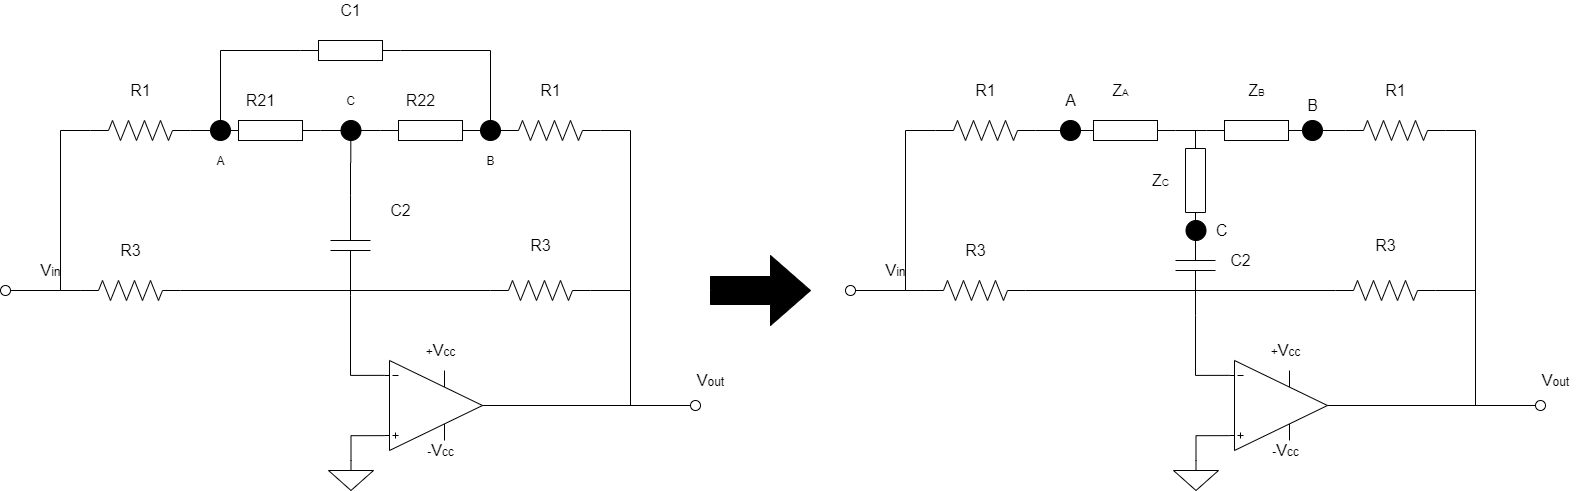
\includegraphics[width=0.9\textwidth]{../Ejercicio4-EcualizadorDeFase/Informe/1cambioEstrella.png}
	\caption{1° Reemplazo - Transformación estrella a triángulo}
	\label{1reemplazo} 
\end{figure}


Para el segundo reemplazo, se reagrupan las impedancias
 de la siguiente manera:

\begin{align}
		Z_{A'} &= R_1 + Z_{A} \\
		Z_{B'} &= R_1 + Z_{B} \\
		Z_{C'} &= \frac{1}{sC_2} + Z_{C}
\end{align}
Se hacen las 
siguientes consideraciones:

\begin{align*}
	Z_{eq'} &= Z_{A'} + Z_{B'} + Z_{C'}
\end{align*}

Consecuentemente, se realiza una transformación de Kenelly, pasando 
de un modelo estrella un triángulo. Obteniéndose las siguientes expresiones:

\begin{align}
	Z_{A'B'} &= \frac{Z_{eq'}}{Z_{C'}} \\
	Z_{B'C'} &= \frac{Z_{eq'}}{Z_{A'}}  \\
	Z_{C'A'} &= \frac{Z_{eq'}}{Z_{B'}} 
\end{align}



\begin{figure}[H]
	\centering
	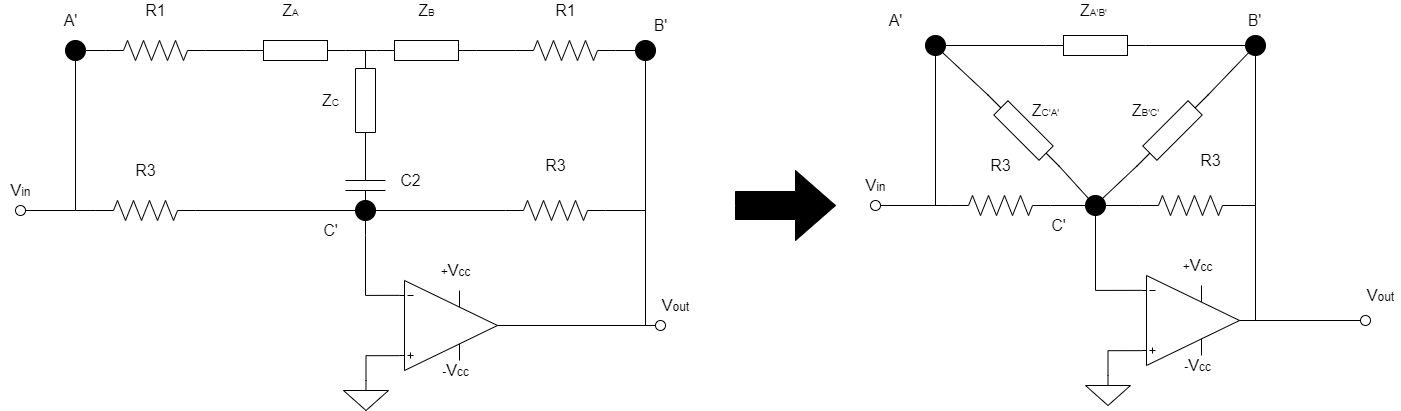
\includegraphics[width=0.9\textwidth]{../Ejercicio4-EcualizadorDeFase/Informe/2cambioTriangulo.png}
	\caption{2° Reemplazo - Transformación estrella a triángulo}
	\label{2reemplazo} 
\end{figure}

Por último simplificamos las impedancias que estaban en paralelo obteniendo un circuito de 3 impedancias mucho más simple de resolver:

\begin{figure}
	\centering
	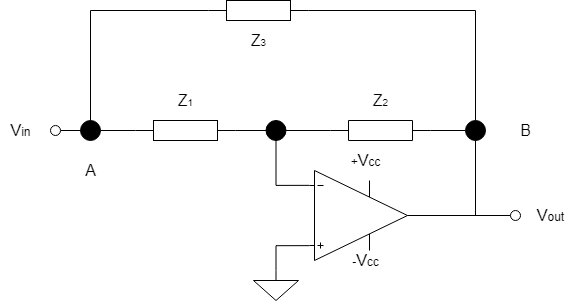
\includegraphics[scale=0.6]{../Ejercicio4_EcualizadorDeFase/Informe/EcFinal.png}
	\caption{Circuito simplificado}
	\label{Cir Final}
\end{figure}

Para no complicar los cálculos se uso el programa Maple
 para poder obtener los resultados finales de los reemplazos, 
 dejando asi las siguientes impedancias:

\begin{align}
		Z_{C''A''} & = Z_{C'A'}//R_3 \\
		Z_{B''C''} & = Z_{B'C'}//R_3
\end{align}
Finalmente, nos queda el circuito simplificado mostrado en 
[\ref{circuito_final}], del mismo se puede despejar la transferencia 
del sistema como:

\begin{align}
	H(\$)=\frac{V_{out}}{V_{in}}=-\frac{Z_{B''C''}}{Z_{C''A''}}
	\label{trans}
\end{align}

\begin{figure}[H]
	\centering
	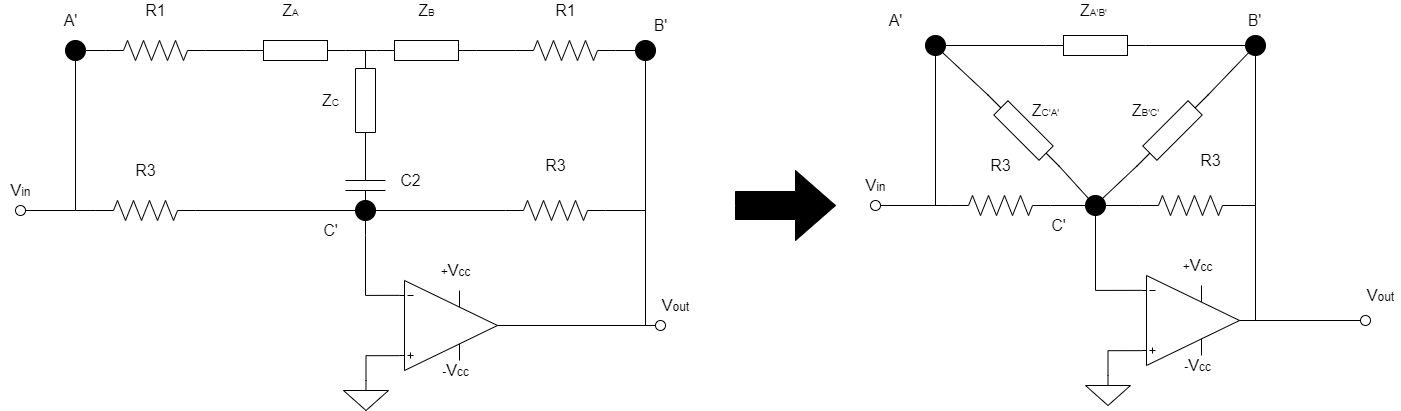
\includegraphics[width=0.9\textwidth]{../Ejercicio4-EcualizadorDeFase/Informe/2cambioTriangulo.png}
	\caption{2° Reemplazo - Transformación estrella a triángulo}
	\label{circuito_final} 
\end{figure}


Trabajando algebráicamente sobre la ecuaci+on




Para facilitar escribir la ecuación se usaron los reemplazos ya mostrados. De la ecuación \ref{ecTransferencia} se puede determinar que la frecuencia de corte del circuito es:


\begin{align}

	\begin{equation}
		\omega_0 = \sqrt{\frac{\beta}{\alpha}}
	\end{equation}
	
	\begin{equation}
		f_0 = \frac{1}{2\pi} . \sqrt{ \frac{2R_1 + R_2 }{ 20 C_2^2 R_1 R_2^2 (L (1-L)) + 100R_1 R_2^2C_2^2 } }
	\end{equation}
	
	\begin{equation}
		f_0 = \frac{1}{2\pi C_2 R_2} \sqrt{ \frac{2 + \frac{R_2}{R_1} }{ 20L(1-L) + 100 } }
	\end{equation}		
	\label{f0sinsimplificar}
	
	\begin{equation}
		f_0 = \frac{1}{2\pi C_2 R_2} \frac{ \sqrt{ \frac{2 + \frac{R_2}{R_1} }{ 1 } } }{ 10 }
	\end{equation}
	\label{f0final}
	
\end{align}

